\section{Our approach}
\subsection{GraphGPS with HIG and IAOTR}
\label{sec:graphgps_hig}
The design of GraphGPS prioritizes flexibility, making it easy to modify and expand upon. This inspired us to integrate HIG-GraphClassification into GraphGPS, combining the concepts of two existing papers. Our focus was on incorporating the Positional Encodings (as shown in Figure \autoref{fig:gps-hig-position}) into the HIG model. However, during the implementation process, we unexpectedly designed what we call Illegal Arithmetic Operation Tensor Replacement (IAOTR). The nodes that would get replaced by an interpolation of feature vectors, get replaced by a very high negative number. This happens because of a division by zero, although the program still executes. IAOTR astonishingly outperforms our HIG-Implementation.

\begin{figure}[!ht]
    \centering
    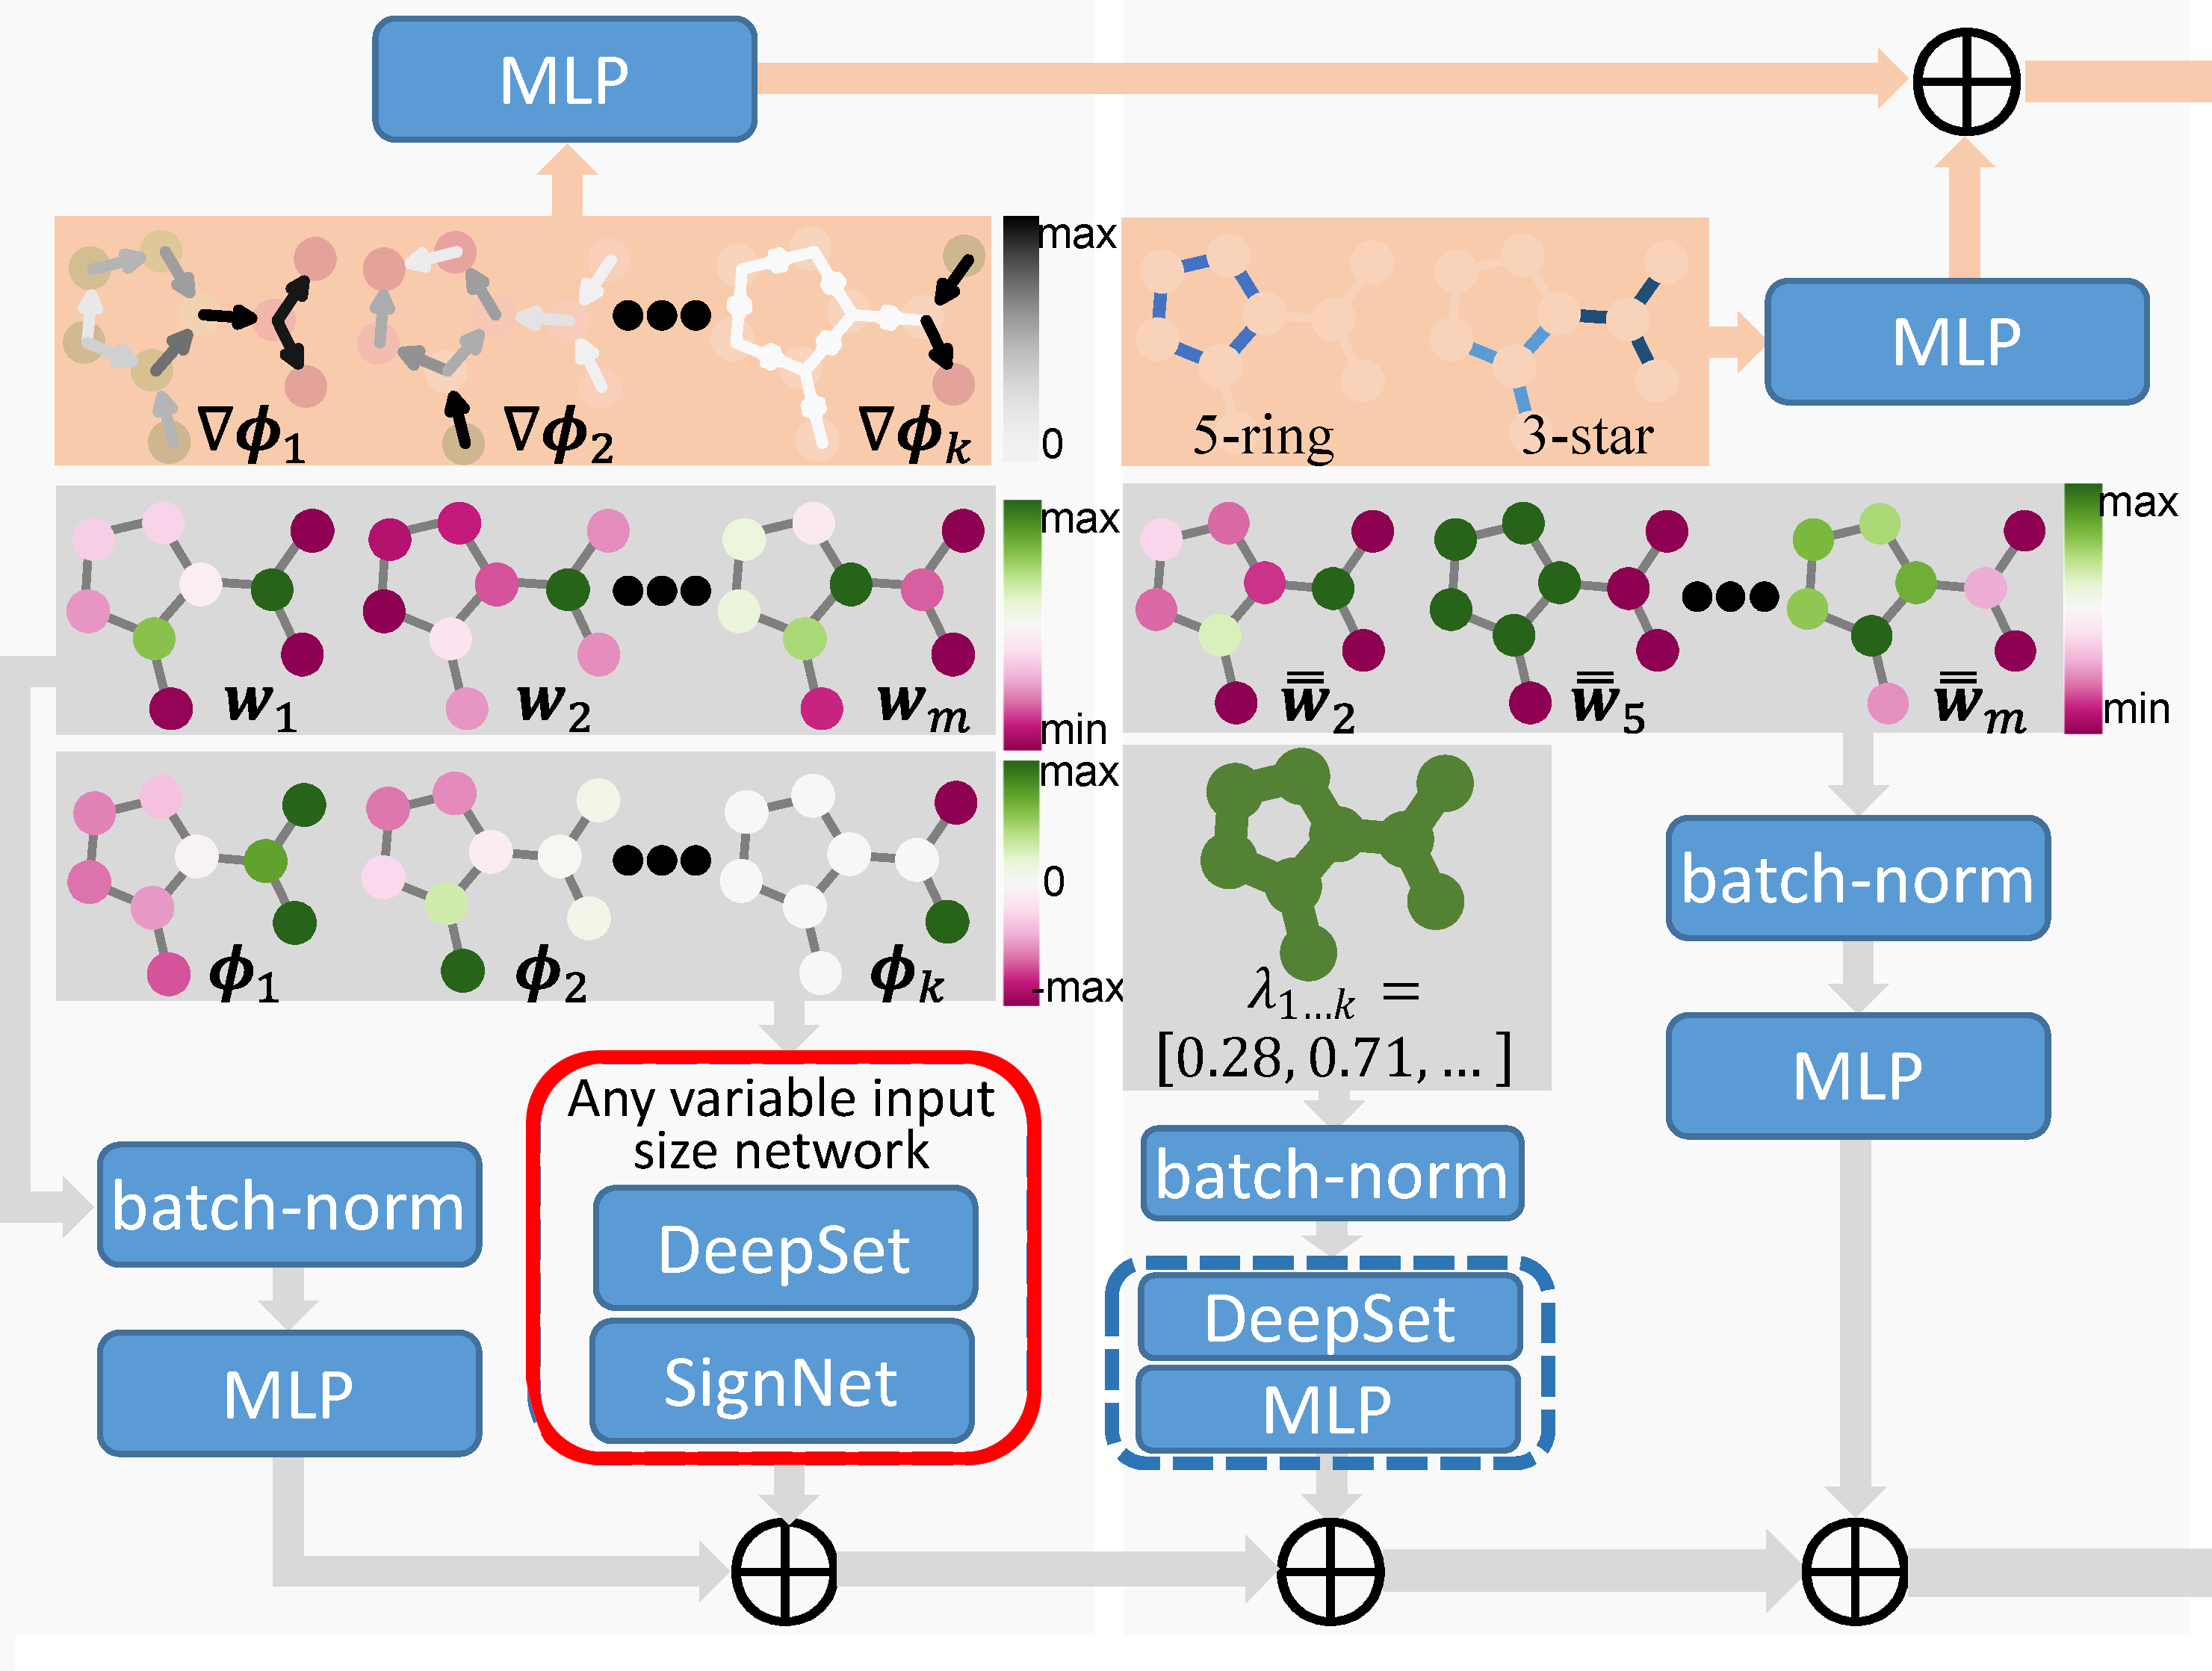
\includegraphics[scale=0.2]{tex/res/gps_hig_position.png}
    \caption{Position of HIG in GraphGPS structure}
    \label{fig:gps-hig-position}
\end{figure}

\subsubsection{Implementation}
The implementation of the heterogeneous interpolation, which involves dropping the feature vector (\autoref{table:node_feature_list}) of several randomly selected nodes and replacing them with an interpolated feature mix, can be found in \autoref{algorithm:HiG_Code_in_GraphGPS}. While our implementation does not include the mixing ratio, we have added a \emph{replacement-p} parameter and a \emph{min\_size} parameter. The \emph{replacement-p} parameter enables us to specify the probability with which the graph replaces a node with an interpolated feature mix. On the other hand, the \emph{min\_size} parameter sets a minimum size for the graph. This is because a smaller graph tends to lose more information if a node is replaced, which could be disadvantageous. Additionally, we have included the \emph{nodes\_replaced} parameter, which allows us to specify the number of nodes that get replaced instead of randomly choosing how many get replaced.

Previously the if-condition in line 15 was never satisfied, which resulted in a division by 0 in line 27. The values of the node feature vector are then replaced by very high negative values. This still executed and lead to the results in \autoref{table:loss_results}.

\begin{minipage}{\linewidth}
    \begin{algorithm}[H]
        %\SetKwSty{text}
        \DontPrintSemicolon
        \SetArgSty{text}
        \SetProgSty{text}
        \SetKw{KwIn}{in}
        \SetKw{KwAnd}{and}

        \SetKwProg{Fn}{def}{}{}
        \If{'HiG' in pe\_types}{
            Replacement\_chance = cfg.posenc\_HIG.Replacement\_p\;
            is\_interpolating = np.random.choice(2, 1, p=[1-Replacement\_chance, Replacement\_chance])[0]\;
            minimum\_node\_size = cfg.posenc\_HIG.minimum\_node\_size\;
            nodes\_replaced = cfg.posenc\_HIG.nodes\_replaced\;
            minimum\_node\_size = max(minimum\_node\_size, nodes\_replaced)\;
            \If{data.num\_nodes > minimum\_node\_size \KwAnd is\_interpolating == 1}{
                rand\_ints = np.random.choice(data.num\_nodes, nodes\_replaced\;
                sum = \{\}\;
                \For{rand\_int \KwIn rand\_ints}{
                    data.x[rand\_int] = 0\;
                    sum[rand\_int] = 0\;
                }
                \For{i,j \KwIn zip(data.edge\_index[0], data.edge\_index[1])}{
                    \If{i.item() \KwIn rand\_ints}{
                        \If{j.item() \KwIn rand\_ints}{
                            continue
                        }
                        relevant\_node = j;
                        data.x[i] = torch.add(data.x[i], data.x[relevant\_node])\;
                        sum[i.item()] += 1\;
                    }
                }
                \For{rand\_int \KwIn rand\_ints}{
                    \If{(sum[rand\_int] ==0)}{
                        continue
                    }
                    data.x[rand\_int] = data.x[rand\_int] / sum[rand\_int]
                }
            }
        }
        \caption{HiG-Code in GraphGPS}
        \label{algorithm:HiG_Code_in_GraphGPS}
    \end{algorithm}
\end{minipage}

\subsubsection{Results}
In \autoref{table:hig_results} are the results of implementing HIG in GraphGPS. For each result in \autoref{table:hig_results} and \autoref{table:loss_results} the model has been executed once with 100 Epochs of Training. The lowest performance was measured when 5 nodes are replaced by an interpolation. For IAOTR the Parameter combination of 0.75 \emph{replacement-p}, 1 node replaced and 20 minimum graph Size performs best. For HIG  this parameter combination also performs best. HIG outperforms IAOTR, the more nodes are replaced. With the \emph{replacement-p} going towards 0.5, IAOTR outperforms HIG.
\begin{table}[ht!]
    \centering
    \begin{tabular}{@{}lllll@{}}
        \toprule
        Model Focus     & Replacement-p & Nodes Replaced & min.graph size & Test-AUC \\ \midrule
        IAOTR           & 1.0           & 1              & 5              & 0.75274  \\
        Replacement-p   & 0.5           & 1              & 5              & 0.77894  \\
                        & 0.1           & 1              & 5              & 0.77033  \\
                        & 0.01          & 1              & 5              & 0.7625   \\
        Nodes Replaced  & 1.0           & 2              & 5              & 0.73967  \\
                        & 1.0           & 3              & 5              & 0.73882  \\
                        & 1.0           & 5              & 10             & 0.71498  \\
        min. graph size & 1.0           & 1              & 10             & 0.76795  \\
                        & 1.0           & 1              & 20             & 0.77084  \\
                        & 1.0           & 1              & 50             & 0.7566   \\
        Combination     & 0.5           & 1              & 20             & 0.77164  \\
                        & 0.75          & 1              & 20             & 0.78321  \\ \bottomrule
    \end{tabular}
    \caption{IAOTR on obgb-molhiv}
    \label{table:loss_results}
\end{table}

\begin{table}[ht!]
    \centering
    \begin{tabular}{@{}lllll@{}}
        \toprule
        Model Focus     & Replacement-p & Nodes Replaced & min.graph size & Test-AUC \\ \midrule
        No HIG          &               &                &                & 0.7710   \\
        HIG             & 1.0           & 1              & 5              & 0.77384  \\
        Replacement-p   & 0.5           & 1              & 5              & 0.76834  \\
                        & 0.1           & 1              & 5              & 0.76564  \\
                        & 0.01          & 1              & 5              & 0.76275  \\
        Nodes Replaced  & 1.0           & 2              & 5              & 0.74348  \\
                        & 1.0           & 3              & 5              & 0.73382  \\
                        & 1.0           & 5              & 10             & 0.72977  \\
        min. graph size & 1.0           & 1              & 10             & 0.76878  \\
                        & 1.0           & 1              & 20             & 0.76636  \\
                        & 1.0           & 1              & 50             & 0.78039  \\
        Combination     & 0.75          & 1              & 20             & 0.7792   \\ \bottomrule
    \end{tabular}
    \caption{Our HIG-Implementation on obgb-molhiv}
    \label{table:hig_results}
\end{table}

\subsubsection{Conclusion}
In conclusion, our experiment revealed that the IAOTR outperformed our HIG-Implementation, despite the unexpected success given that the code was not intended to function in this way. We believe that this is due to the IAOTR  being more effective in preventing overfitting. On the other hand, when more nodes are replaced, HIG's performance surpasses that of the IAOTR, which may be due to the latter losing too much information at each node. Interestingly, our results also suggest that IAOTR on smaller molecules may eliminate crucial information, which is why HIG has a better performance in the standard setting.

Our explanation for why IAOTR works is because the high negative value gets replaced by 0 in a ReLU function that the standard GraphGPS \cite{2023graphgps} uses.
Further research into IAOTR could shed more light on this phenomenon and offer insights into optimizing molecular representation learning.
